% CONCLUSIONI

\chapter{Conclusioni}\label{chap:conclusions}
\section{Valutazione del prodotto finale}
L’applicazione \emph{Teamwork} sviluppata nei due mesi di stage soddisfa pienamente le aspettative dell’azienda, in quanto non pensavano di arrivare ad avere in mano un prototipo con tutte le funzionalità principali. \\
Questo ha confermato all'azienda l'effettiva utilità di un'applicazione mobile di chat da integrare nella \emph{suite Zextras}. Infatti il progetto \emph{Teamwork} verrà portato avanti senza applicare cambiamenti drastici dell'architettura, a partire dal codice sviluppato nei mesi di stage.\\
La figura \ref{sec:valutazione} rappresenta tre \emph{screen} dell'applicazione finale (rispettivamente \emph{login}, \emph{buddylist} e\emph{ chat page}) che possono essere confrontati con la figura \ref{subsec:wireframe} che rappresenta i \emph{wireframe} progettati.
\begin{figure}[H] 
	\centering
	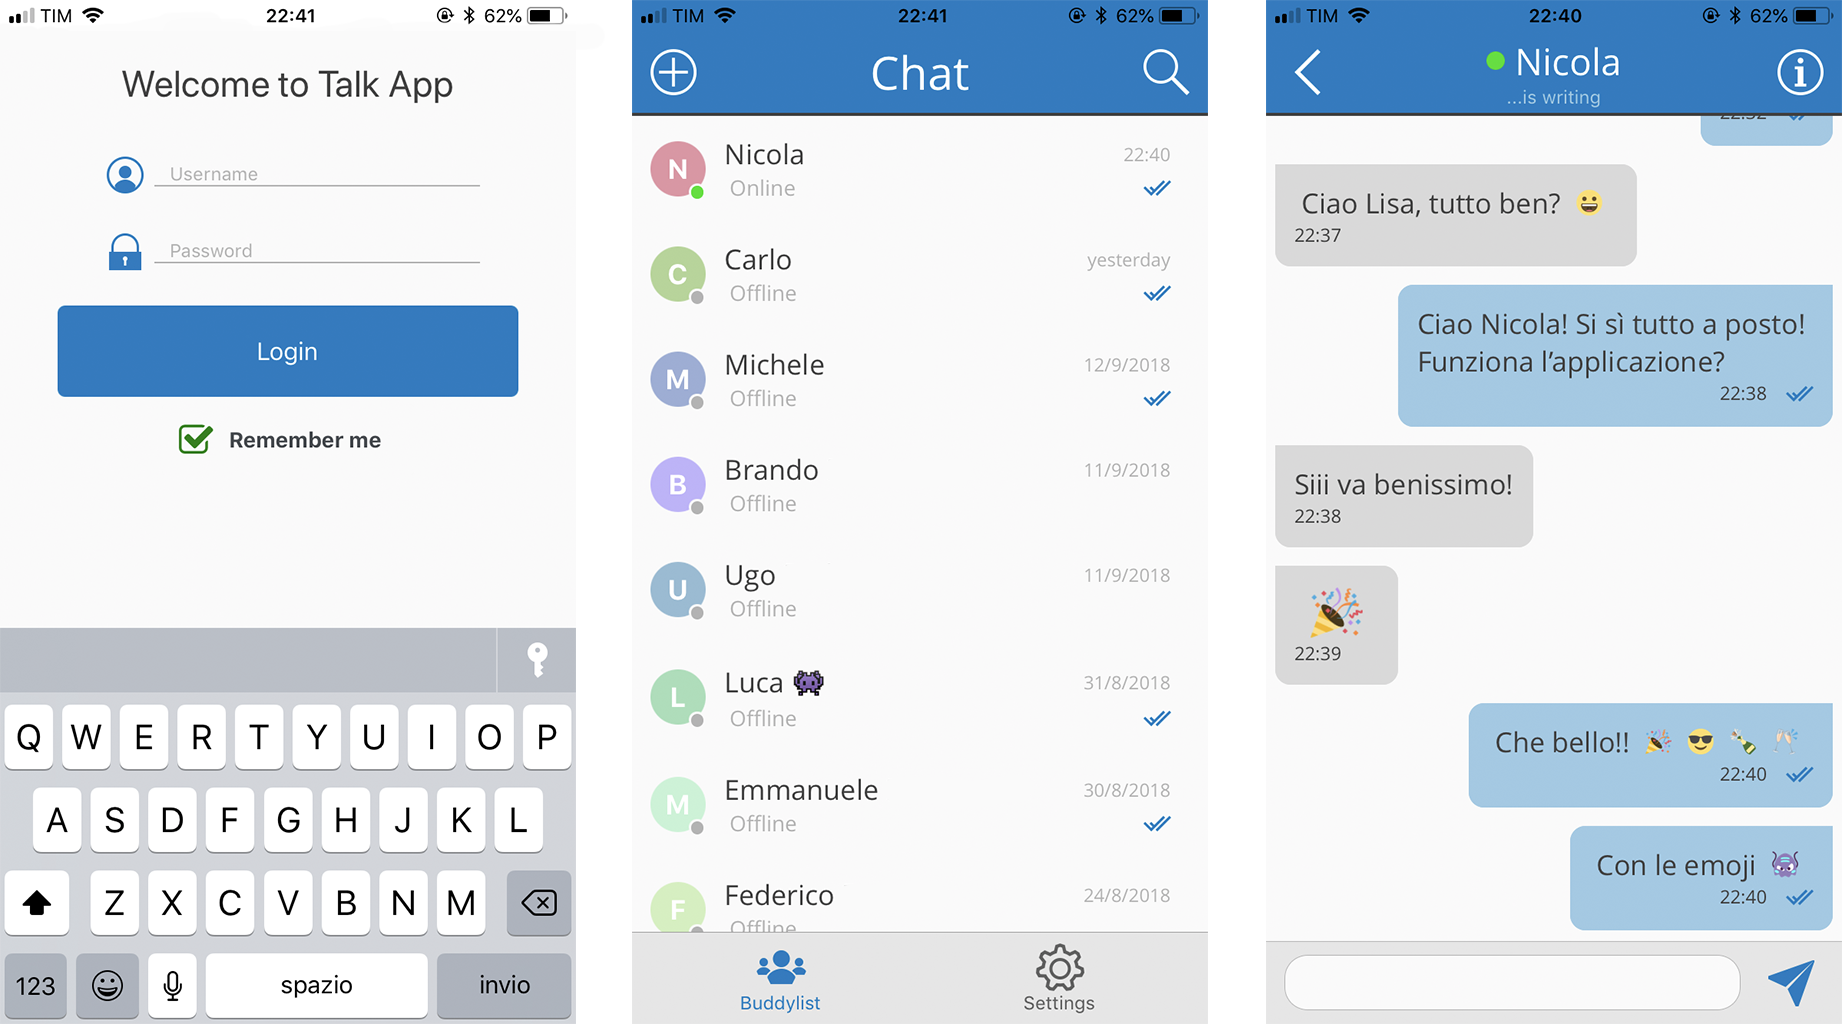
\includegraphics[scale=0.45]{screen}
	\caption{Screen pagina di login, buddylist e chat page.}
	\label{sec:valutazione}
\end{figure}
Per quanto riguarda l'interfaccia grafica sono molto soddisfatta del risultato ottenuto in quanto segue perfettamente le linee guida fornite dall'azienda. \\
Personalmente ritengo il prodotto sviluppato un ottimo prototipo della possibile chat della suite, ma la ritengo ancora lontana dall'essere una versione rilasciabile e testabile da utenti esterni principalmente per due motivi:
\begin{itemize}
	\item le funzionalità implementate non sono abbastanza numerose da coprire i bisogni che dovrebbe soddisfare questo tipo di applicazione;
	\item essendo una suite di prodotti utilizzati in ambiente lavorativo è necessario assicurare una certa sicurezza nella comunicazione dei dati e nella connessione ai server, criptando i messaggi all'invio. Ciò non è stato però previsto nello stage.
\end{itemize}

\section{Valutazione framework e librerie utilizzate}
L'obbiettivo di questo progetto di stage, oltre ad avere un prototipo funzionante dell'applicazione, era quello di validare delle tecnologie ancora non utilizzate dall'azienda per capire se fossero effettivamente utili allo sviluppo di futuri progetti. \\
Sebbene abbia ancora molto da imparare su queste tecnologie per poterne giudicare pregi e difetti in maniera critica, ritengo adeguato effettuare una valutazione a posteri del compimento del progetto.
\subsection{Valutazione React Native}
Per realizzare l'interfaccia utente delle ultime \emph{zimlet} sviluppate dall'azienda si è utilizzato ReactJS, libreria JavaScript che ha permesso di migliorare lo sviluppo e la gestione dei dati rispetto alla precedente tecnologia utilizzata specifica per \emph{Zimbra}. \\
Per la realizzazione di applicazioni mobile è disponibile una sua variante, React Native, che, nonostante le differenze, presenta una struttura simile. \\
Proprio per mantenere una certa continuità è stato deciso di testare le funzionalità di React Native in questo progetto. \\
In base all'esperienza di sviluppo avuta ho potuto valutare React Native in base a vari punti:
\subsubsection{App multipiattaforma}
React Native permette lo sviluppo di applicazioni mobile sia Android che iOS utilizzando JavaScript. In questo modo non è necessario sviluppare due versioni dell'applicazione in due linguaggi differenti per poter pubblicare l'app nei due \emph{store} (App Store e Google Store). \\
Ovviamente questa integrazione presenta anche degli aspetti negativi da valutare. Innanzitutto le piattaforme native Android ed iOS presentano molte differenze e tentare di generalizzare i comportamenti di tutti i componenti nativi risulta impossibile. Per questo motivo non sono implementati tutti i componenti che avremmo a disposizione nei due ambienti di sviluppo nativi e. inoltre, non è detto che un componente si comporti in modo uguale sui diversi sistemi operativi per mobile. \\
In secondo luogo React Native crea un livello di astrazione al di sopra dell’applicazione che può essere meno performante di un dialogo diretto tra applicazione nativa e sistema operativo.
\subsubsection{Virtual DOM}
Per accedere e aggiornare dinamicamente il contenuto, la struttura e lo stile dei documenti nel \emph{client web} e nelle applicazioni che utilizzano \emph{WebView} si utilizza il \emph{\textbf{D}ocument \textbf{O}bject \textbf{M}odel} (\acrshort{DOM}), una forma di rappresentazione dei documenti strutturati, che tenta di renderli neutrali rispetto alla lingua e alla piattaforma. React Native, invece, utilizza il Virtual DOM che crea una struttura dei dati\emph{ in-memory}: lavorando per differenza aggiorna in modo efficiente la DOM visualizzata dal browser. In tal modo vengono renderizzati solamente i componenti che vengono modificati e non tutta la pagina.
\subsubsection{JSX e CSS}
Il framework utilizza JSX come linguaggio di \emph{markup} e uno pseudo CSS per lo stile.
Per quanto riguarda JSX il suo scopo è definire una sintassi concisa e familiare per la definizione delle strutture dell'albero con i relativi attributi per ogni nodo. Risulta molto intuitivo in quanto ha una sintassi simil XML ed è facilmente gestibile in quanto possono essere implementate al suo interno funzioni JavaScript.\\
Per gestire lo stile di ogni componente, invece,  si utilizza un simil CSS (in formato JSON) che risulta limitato nelle dichiarazioni. Non è possibile quindi utilizzare estensioni come SCSS e riutilizzare lo stylesheet web per intero. 

\subsection{Valutazione Expo}
Il tool di sviluppo per applicazioni in React Native Expo è una tecnologia completamente nuova per l'azienda, consigliata da un consulente esterno. Ho raccolto i principali benefici e svantaggi dell'utilizzo di esso.\\
Aspetti positivi:
\begin{itemize}
	\item semplifica delle operazioni comuni che non sono gestite dai componenti di React Native introducendo dei nuovi componenti Expo;
	\item velocizza di molto i tempi di \emph{testing} su \emph{device} fisici, in quanto Expo propone \emph{build} automatiche nei propri server che possono essere scaricate su qualsiasi \emph{device} tramite un \emph{link} alla \emph{build};
	\item riduce la complessità di creazione di file \texttt{.apk} e \texttt{.ipa} in quanto crea le \emph{build} nei propri server e gestisce le certificazioni in autonomia.
\end{itemize}
Aspetti negativi:
\begin{itemize}
	\item l'interazione tra Expo e React Native Debugger ha riscontrato non pochi problemi, che causavano spesso l'interruzione dei servizi Expo;
	\item Expo client risulta ancora molto instabile causando \emph{crash} dell'applicazione.
\end{itemize}
\newpage
\section{Valutazione personale dell'esperienza di stage}
Anche se il mio percorso di studi precedente all'Università non mi ha mai portato allo studio di discipline informatiche ho deciso di affacciarmi a questo mondo che tanto mi affascinava iscrivendomi al corso di Informatica all'Univesità. \\
Sebbene impegnativo, soprattutto per chi, come me, non aveva conoscenze tecniche pregresse, mi è stato subito chiaro dell'ottima scelta fatta. Nei tre anni di lezione ho potuto apprendere, oltre alle conoscenze tecniche, un metodo di ragionamento, ad affrontare e risolvere problemi, ad analizzare situazioni e dati e, per me importantissimo, ad applicare la mia creatività in tutto ciò.\\
In questo stage di fine percorso mi è stata data la possibilità di mettere in pratica tutte le abilità fin ora apprese solo in teoria. Ho potuto dimostrare all'azienda e, soprattutto, a me stessa, di avere le capacità di portare avanti un progetto, di saper gestire il lavoro e di mettere del mio in ogni fase del progetto.\\
Oltre ad avermi dato la carica per affrontare a testa alta il mondo del lavoro mi è stato utilissimo per le conoscenze tecniche ottenute. Ho potuto imparare un nuovo linguaggio di programmazione, utilizzato dei \emph{framework} e librerie utilissime in molti ambiti e ottenuto dimestichezza con vari strumenti di gestione del lavoro. Tutto questo insieme al fatto che ho potuto integrarmi in un team di sviluppo, comprendendo meglio dinamiche e rapporti molti differenti da quelli dell'Università.\\
Sebbene sia ancora alle prime armi ed abbia ancora molto da apprendere mi sento di dire che l'esperienza di stage è riuscita a far concludere il mio percorso di studi della laurea triennale con entusiasmo, dandomi la carica e la voglia di continuare il percorso di studi affrontando la laurea magistrale in Informatica e, allo stesso tempo, continuando il progetto iniziato presso l'azienda.